

\documentclass{beamer}

\usepackage[utf8]{inputenc}
\usepackage[numbers]{natbib}
\usepackage{centernot}

\newcommand{\defeq}{\coloneqq} % :=
\newcommand{\eqdef}{\eqqcolon} % =:

\renewcommand{\P}{\mathbb{P}} % probability P
\newcommand{\E}{\mathbb{E}} % expectation E
\newcommand{\V}{\mathbb{V}}
\newcommand{\bs}{\boldsymbol}
\newcommand{\IX}{\bs{1}}

\newcommand{\eps}{\epsilon}

\DeclareMathOperator*{\argmin}{arg\,min}
\DeclareMathOperator*{\argmax}{arg\,max}

\mode<presentation> {

\usetheme{Warsaw}
%\usecolortheme{Dolphin}
}
\expandafter\def\expandafter\insertshorttitle\expandafter{%
	\insertshorttitle\hfill%
	\insertframenumber\,/\,\inserttotalframenumber}
\usepackage{graphicx} % Allows including images
\usepackage{booktabs} % Allows the use of \toprule, \midrule and 
\usepackage{wrapfig}
\usepackage{subcaption}
\captionsetup{subrefformat=parens}

\title[Reinforcement Learning]{ Reinforcement Learning for Blackjack} % The short title appears at the bottom of every slide, the full title is only on the title page

\author{Benjamin Allévius, Sebastian Rosengren, Erik Thorsén} % Your name
\institute[SU] % Your institution as it will appear on the bottom of every slide, may be shorthand to save space
{
Department of Mathematics, Stockholm University
}
\date % Date, can be changed to a custom date

\begin{document}
	
\begin{frame}
	\titlepage % Print the title page as the first slide
	\centering
\end{frame}


\section{Introduction}

\begin{frame}{Purpose}
	Use reinforcement learning to train an \textit{agent} to play blackjack\newline
	
	Investigate Learning capabilities of the framework\newline
		
	Compare two different representations of the state space
\end{frame}

\begin{frame}{Blackjack}
\begin{itemize}
	\item One player against the dealer, with player staking one unit on each hand;
	\item two actions possible: ask for another card, or stay;
	\item cards 2--10 counts as their numerical value, suites counts as 10, and ace counts as either 1 or 11 depending on whichever is best. If an ace can be counted as 11 without player going bust it is known as a \textit{usable} ace, the same goes for the dealer.
\end{itemize}
\end{frame}

\begin{frame}{Blackjack}
	The goal of the player is to beat the dealer in one of the following ways
	\begin{itemize}
		\item Get 21 points on the first two cards, knows as a blackjack, without a dealer blackjack. \textbf{Net profit}: 1.5 times stake;
		\item Reach a final score higher than the dealer without exceeding 21. \textbf{Net profit}: stake;
		\item Dealer gets points exceeding 21 and player does not. \textbf{Net profit}: stake.
	\end{itemize}
\end{frame}

\begin{frame}{Blackjack as a Markov Decision Process}
	Recall the building blocks of a Markov Decision Process:
	\begin{enumerate}[(i)]
		\item  $S$ a finite space of \textit{states}
		\item  $A$ a finite space of \textit{actions}
		\item  $R$ a finite space of \textit{rewards}
		\item  $P_a(s,s')$ a transition probability function defined for all  $(s,a,s') \in S\times A \times S$
		\item  $r(s,a)$ the immediate or expected immediate reward of taking action $a$ in state $s$.
	\end{enumerate}
\end{frame}

\begin{frame}{Blackjack as a Markov Decision Process}
We represent the state space $S$ in two different ways.
First, let
\begin{align*}
&S = \{  (s_{p1},\ldots,s_{p10},\Sigma_{d})  \} \\
&= \{ (\text{(number of different cards of each type), dealer card sum}) \}.
\end{align*}

Secondly, let

\begin{align*}
S = \{  (\Sigma_p, a_p, \Sigma_d )  \}=\{  (\text{card sum, usable ace, dealer card sum})  \}
\end{align*}
This representation does not yield a \textit{stationary} Markov process since
\begin{align*}
	&s_0 = (21, 1, x),\qquad s_5 = (21,1,x)\\
	&r(s_0, \text{stay}) = 1.5 \neq r(s_5, \text{stay}). 
\end{align*}


\end{frame}



\section{Implementation}

\begin{frame}{Q-Learning for Blackjack}
In a given state, do we \emph{hit} or \emph{stand}? 
\begin{itemize}
  \item Action-value function for policy $\pi$: $q_{\pi} = \E_{\pi}[R_{T} | S_t = s, A_t = a]$, $T>t$ and $S_T$ terminal.
  \item Estimate $q$ for the optimal $\pi$ by the \emph{learned} action-value function
    \begin{align*}
      Q(s_t,a_t)  &\leftarrow (1-\alpha_t(s_t,a_t))Q(s_t,a_t) \\
                  &~+ \alpha_t(s_t,a_t)[ r_{t+1} + \max_{a \in A} Q(s_{t+1},a) ]
    \end{align*}
  \item $Q$ approximates optimal $q_*$ \emph{independent of policy}.
\end{itemize}
\end{frame}

\begin{frame}{Q-Learning Implementation}
Blackjack has discrete and finite action and state spaces $\Rightarrow$
algorithm guaranteed to converge if
\begin{itemize}
        \item Learning rate $\alpha_t(s,a) \in (0, 1]$ is such that
          \begin{align*}
            \sum_t \alpha_t(s,a) = \infty \text{ and } \sum_t \alpha^2_t(s,a) < \infty
          \end{align*}
          for each pair $(s, a)$.
        \item All state-action pairs are visited infinitely often (in the limit).
\end{itemize}
To do this, we set
\begin{itemize}
  \item $\alpha_t(s,a) = \frac{1}{\#[(s=s_t,a=a_t)]^{0.77}} \text{ \citep[see][]{EvenDar2003}}$
  \item $\epsilon_t(s) = \frac{0.5}{\#[(s=s_t)]}$ \text{ ($\epsilon$-greedy with decay)}
\end{itemize}
\end{frame}

\begin{frame}{Blackjack Learning Environment}
To apply Q-learning to Blackjack, we used the OpenAI Gym environment (\url{https://gym.openai.com/}).
In doing so we
\begin{itemize}
  \item Fixed the `broken' default state space.
  \item Implemented the extended state space.
  \item Extended the environment from an infinite deck to an arbitrary number of decks.
\end{itemize}
Our code will be made publicly available, possibly through OpenAI Gym.
\end{frame}

\section{Results}

\begin{frame}{Outline of simulation study}

\begin{itemize}
  \item Let two agents learn on two different state spaces, ''hand'' \& ''sum''
  \item Both spaces have the same amount of decks in play
  \item Agents start of \textit{exactly} the same, same q-learning algorithm,  etc. 
  \item For each state/action, track the avg. return (and values of $q$). 
  \item Agents get to play $10^7$ episodes of blackjack. 
\end{itemize}

\end{frame}

\begin{frame}{Avg. return}

\begin{figure}
\begin{tabular}{cc}
\centering
 \begin{subfigure}[b]{0.48\textwidth}
  	 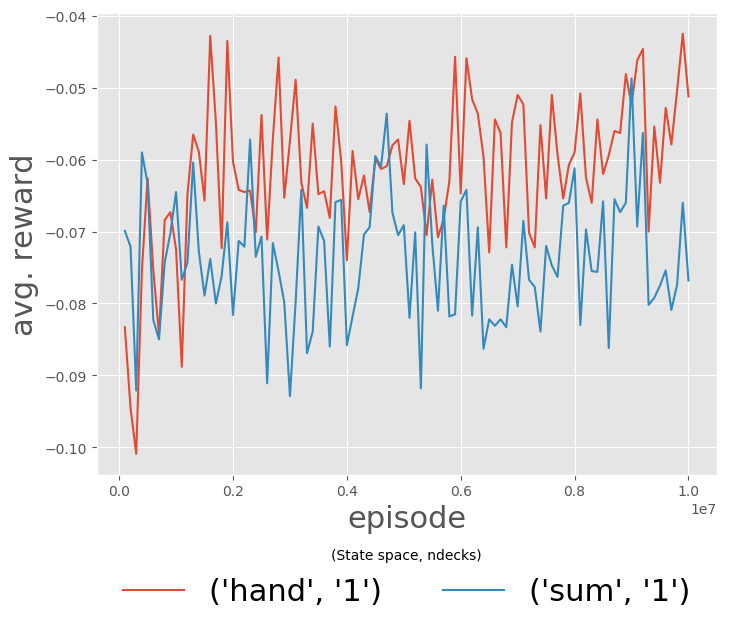
\includegraphics[width=\textwidth]{../report/figures/avgReturnEp_ndeck1.png}
   % .: 0x0 pixel, 0dpi, 0.00x0.00 cm, bb=
   \caption{Avg. return with 1 deck}
 \end{subfigure}
 &
 \begin{subfigure}[b]{0.48\textwidth}
  	 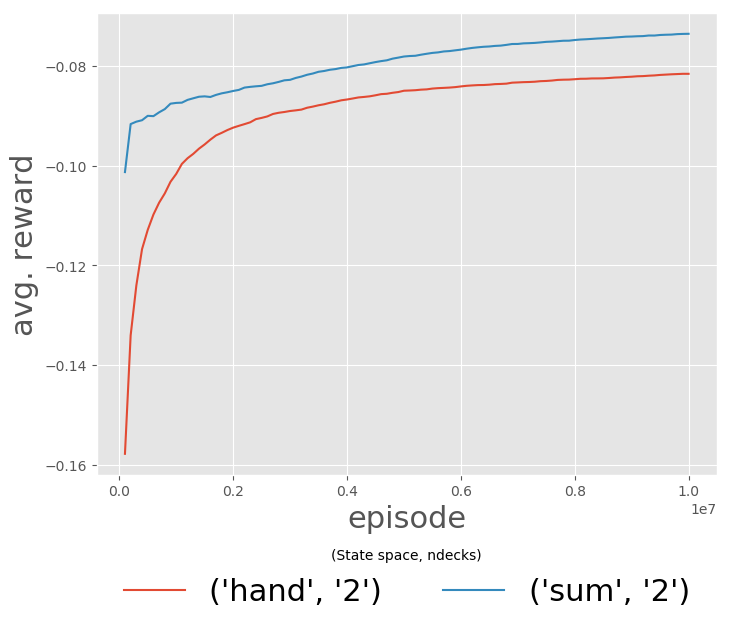
\includegraphics[width=\textwidth]{../report/figures/avgReturnEp_ndeck2.png}
   % .: 0x0 pixel, 0dpi, 0.00x0.00 cm, bb=
   \caption{Avg. return with 2 decks}
 \end{subfigure}
\end{tabular}
\end{figure}

\end{frame}

\begin{frame}{Number of visited states, learning time}
\begin{table}[h!]
\centering
 \begin{tabular}{c|cc|cc}
  \# decks & $\#S_{hand}$ & $t_{hand}$ & $\#S_{sum}$ &  $t_{sum}$  \\
  \hline 
  $1$ & $7651$ & $1510.681$ & $641$ & $1003.765$ \\
  $2$ & $38266$ & $1565.314$ & $677$ & $1079.656$ \\
  $8$ & $70034$ & $1606.944$ & $695$ & $1079.626$ \\
  $\inf$ & $70307$ & $1636.044$ & $671$ & $1097.971$ 
 \end{tabular} 
 \caption{The number of explored states $\#S$ and the training time $t$ (seconds) for a given number of decks in play and its respective state space.\label{tab:state_visited}}
\end{table}
\end{frame}

\section{Summary}

\begin{frame}{Discussion}

\begin{itemize}
 \item Q-learning on two representations of the state space of blackjack
 \item Performance? Simpler representation is better (Cardinality of the larger representation is immense!)
 \item Longer training time $\rightarrow$ results might be different 
 \item Extensions: Several agents, memory to the agent $\rightarrow$ counting cards? 
\end{itemize}

\end{frame}

\begin{frame}{References}
\bibliographystyle{apalike}
\bibliography{references}
\end{frame}
\end{document}



